%! TEX root = 'main.tex'

\section{Background}
\label{sec:background}

%In this section , we talk about the background knowledge of kernel TOCTOU vulnerability, how it happens. Also SMAP feature of Intel processor, how to leverage it as the core mechanism to prevent kernel TOCTOU attacks.  

%Time Of Check to Time Of Use is a class of software bug caused by changes in a system between the checking of a condition and the use of the results of that check. Normally some data changes, such as an variable. In general, it's an example of race conditions.

%This issue has been addressed by many research work ~\cite{dean2004fixing}~\cite{borisov2005fixing}. A classic TOCTOU is similar to the following pseudocode:

TOCTOU is a vulnerability class caused by changes in a system between checking a condition and using that check results. Typically, a variable changes after it passes the sanity check. Many previous research works has addressed this issue~\cite{dean2004fixing}~\cite{borisov2005fixing}. ~\autoref{fig:toctou} shows a classic TOCTOU issue.

\begin{figure}[th]
	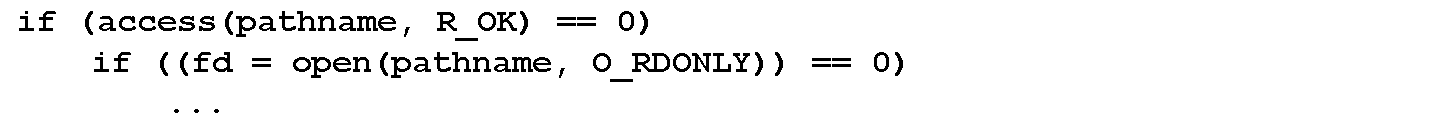
\includegraphics[width=0.47\textwidth]{figures/toctou}
	\centering
	\caption{The gap between access() and open() leaves the attack time window for the attacker to make changes in the file system.}
	\label{fig:toctou}
\end{figure}

%\begin{lstlisting}[basicstyle=\small,style=redkeyword]
%\begin{lstlisting}[style=code]
%if (access(pathname, R\_OK) == 0)
%    if ((fd = open(pathname, O\_RDONLY)) == 0) ...
%\end{lstlisting}



Assume this code piece belongs to a setuid program. It first validates that the ``pathname'' is readable, and if so, open the file for reading. However, the attacker can change the file system between the two system calls to trick the setuid program into opening a file that it should not.

Essentially, TOCTOU vulnerability occurs between security boundaries. The less privileged sector deceives the privileged sector to do unexpected actions. The non-atomic or repeated operation on the same variable is the root cause.

\hb{Dont understand this pragraph, maybe you can clearly describe the attack, like how it could open another file and why}

\subsection{Kernel-level TOCTOU Vulnerability}


TOCTOU also happens in the operating system kernel, inside system calls. For the rest of the paper, we name it kernel-level TOCTOU. An operating system provides services such as ``program execution'', ``I/O operation'', ``file system'' to the programs on a service-client basis. When requesting a system service, the programs provide parameters, and how to invalidate them, keep them consistent during the system call is the kernel's responsibility. However, due to various reasons, the kernel may not fully decouple with the user-mode components. Therefore, directly accessing user-mode variables from the kernel is not uncommon to some operating systems, especially Windows.

When the kernel repeatedly reads the same user-mode address, so-called double fetches, this type of behavior may lead to severe issues, typically local privilege escalation vulnerability. The malicious program first has a benign variable in userspace, then uses another thread to change the variable to bypass the parameter sanity check or introduce errors such as a buffer overflow in-between the kernel's two fetches. The time window between the two kernel fetches may be as short as several instructions,  but with careful design, the race condition created between the kernel and the user program makes it feasible, especially on a multi-processor system.



The correct way of handling user-mode parameters is to ``capture'' (copy) them first, then use the kernel copy for the rest of the system call. It is better to put such standard code into gateway functions for the kernel and drivers, such as those used in the Linux kernel, \texttt{copy\_to\_user()}, and \texttt{copy\_from\_user()}.

However, due to mistakenly repeated operations on user parameters, the kernel-level TOCTOU still widely exists among operating systems already taking the aforementioned method. ~\autoref{table:cves} lists a portion of recent kernel-level TOCTOU vulnerabilities.

\begin{center}
\begin{table}[ht]
%\singlespacing
%\scalebox{0.8}{
\small
\caption{Recent vulnerabilities categorized as race condition or time-of-check-to-time-of-use in the CVE database.}
\label{table:cves}
\centering
	\begin{tabular}{@{}>{\raggedright\arraybackslash}m{2.35cm}@{}|
			@{}>{\centering\arraybackslash}m{1.35cm}@{}|
			@{}>{\centering\arraybackslash}m{2.35cm}@{}|
			@{}>{\centering\arraybackslash}m{1.25cm}@{} } 
\hline
CVE-ID & Affected System & CVE-ID & Affected System \\ %[0.5ex]
\hline
CVE-2008-2252  & Windows & CVE-2016-5728 & Linux \\
CVE-2013-1280  & Windows & CVE-2016-6130 & Linux \\
CVE-2018-7249  & Windows & CVE-2020-9796 & macOS \\ 
CVE-2020-9839  & macOS   & CVE-2020-9990 & macOS \\
CVE-2016-10439 & Android & CVE-2016-7624 & macOS \\
CVE-2016-10383 & Android & CVE-2017-7115 & iOS \\

CVE-2020-5967  & Nvidia  & CVE-2020-8680 & Intel \\
\hline

\end{tabular}
\end{table}
\end{center}



%Notice that large part of the vulnerabilities of this table (from CVE-2013-1248 to CVE-2013-1280) are fixed in one Windows patch MS13-016, they are found by Gynvael Coldwind and Mateusz Jurczyk with Google Security Team. Due to the nature of kernel TOCTOU, it's difficult to exposure them in normal ways of testing or daily usage, until certain pattern and methods are found~\cite{jurczyk2013identifying}.  

%\begin{comment}
%\begin{figure}[th]
%  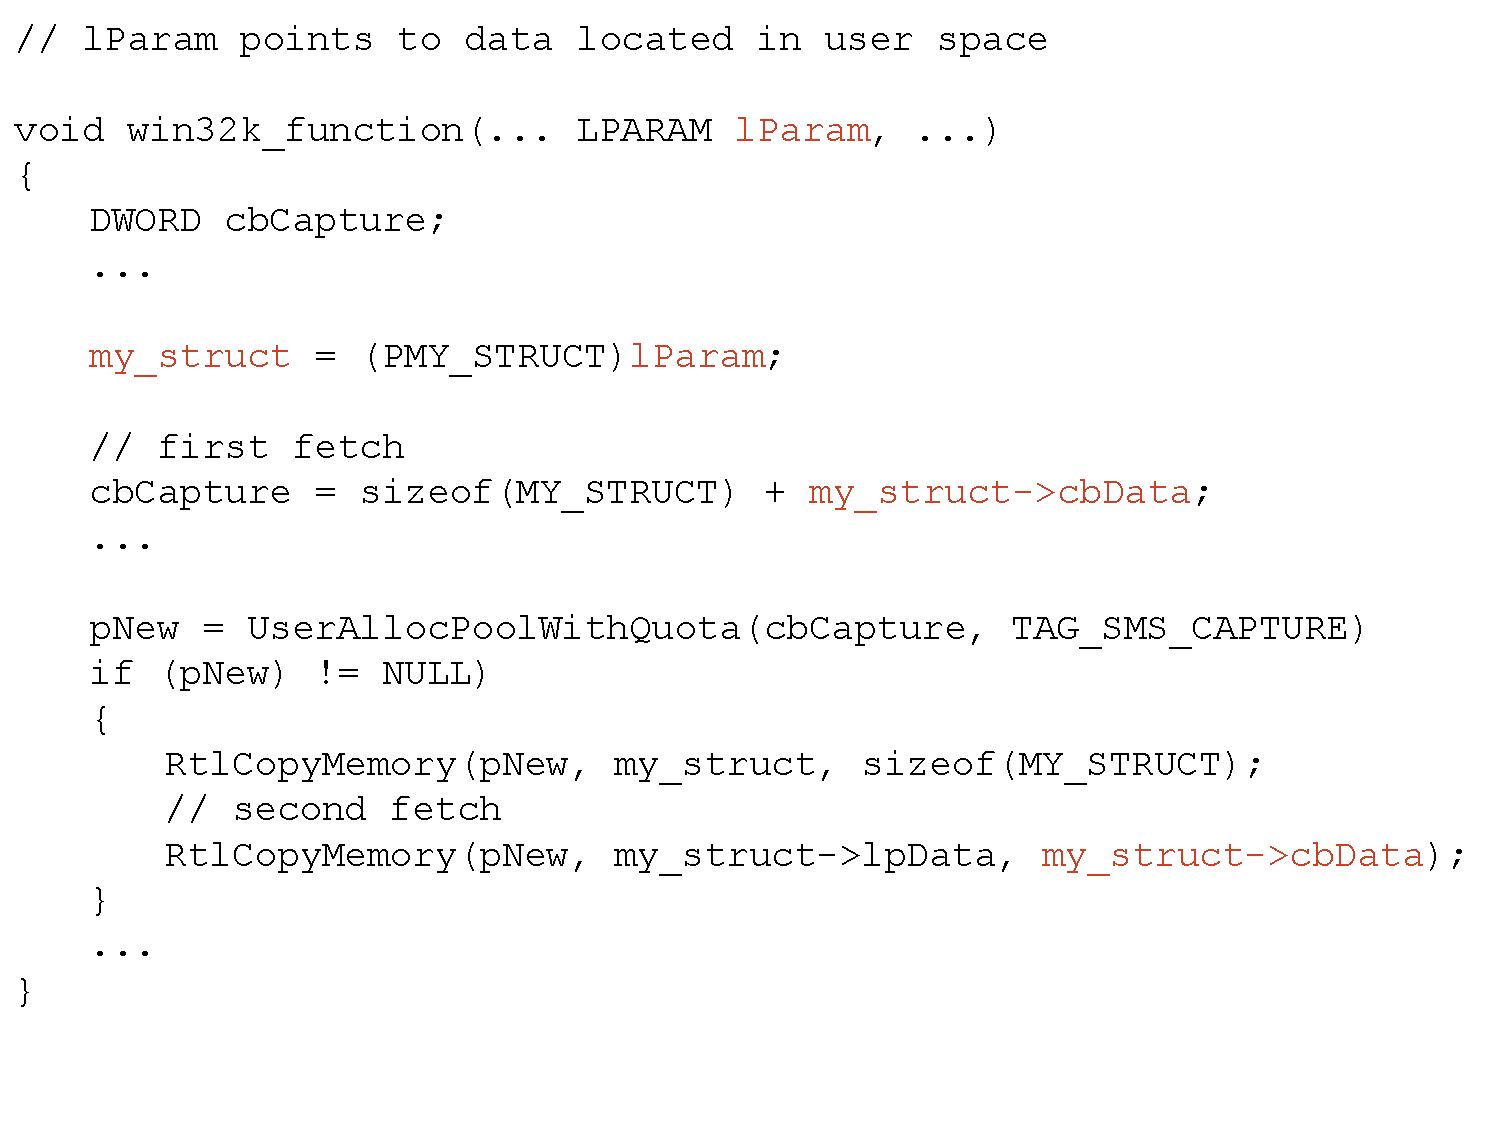
\includegraphics[width=0.47\textwidth]{toctouexample}
%  \centering
%  \caption{Sample code which has TOCTOU vulnerability. Data with in user space is referenced twice during a kernel pool allocation and data copying. ~\cite{jurczyk2013identifying}~\cite{ms08061}}
%  \label{fig:toctouexample}
%\end{figure}
%\end{comment}


%lst:vulnerablecode
%\begin{lstlisting}[style=code,caption={An snippet of Windows device driver code that mimic the vulnerability that fixed in ms08-061. The vulnerable user-mode variable is marked in red.}\label{lst:vulnerablecode}, captionpos=b]
%// lParam points to data located in user space
%void win32k_function(... LPARAM @lParam@, ...) 
%{
%    DWORD cbCapture;
%    ...
%    @my_struct@ = (PMY_STRUCT)@lParam@;
%
%    // first fetch
%    cbCapture = sizeof(MY_STRUCT) + @my_struct->cbData@;  
%    ...
%    pNew = UserAllocPoolWithQuota(cbCapture, TAG_SMS_CAPTURE)
%    if (pNew != NULL) 
%    {
%        RtlCopyMemory(pNew, my_struct, sizeof(MY_STRUCT);
%        // second fetch
%        RtlCopyMemory(pNew, my_struct->lpData, @my_struct->cbData@);   
%    }
%    ...
%}
%
%\end{lstlisting}


\begin{figure}[th]
	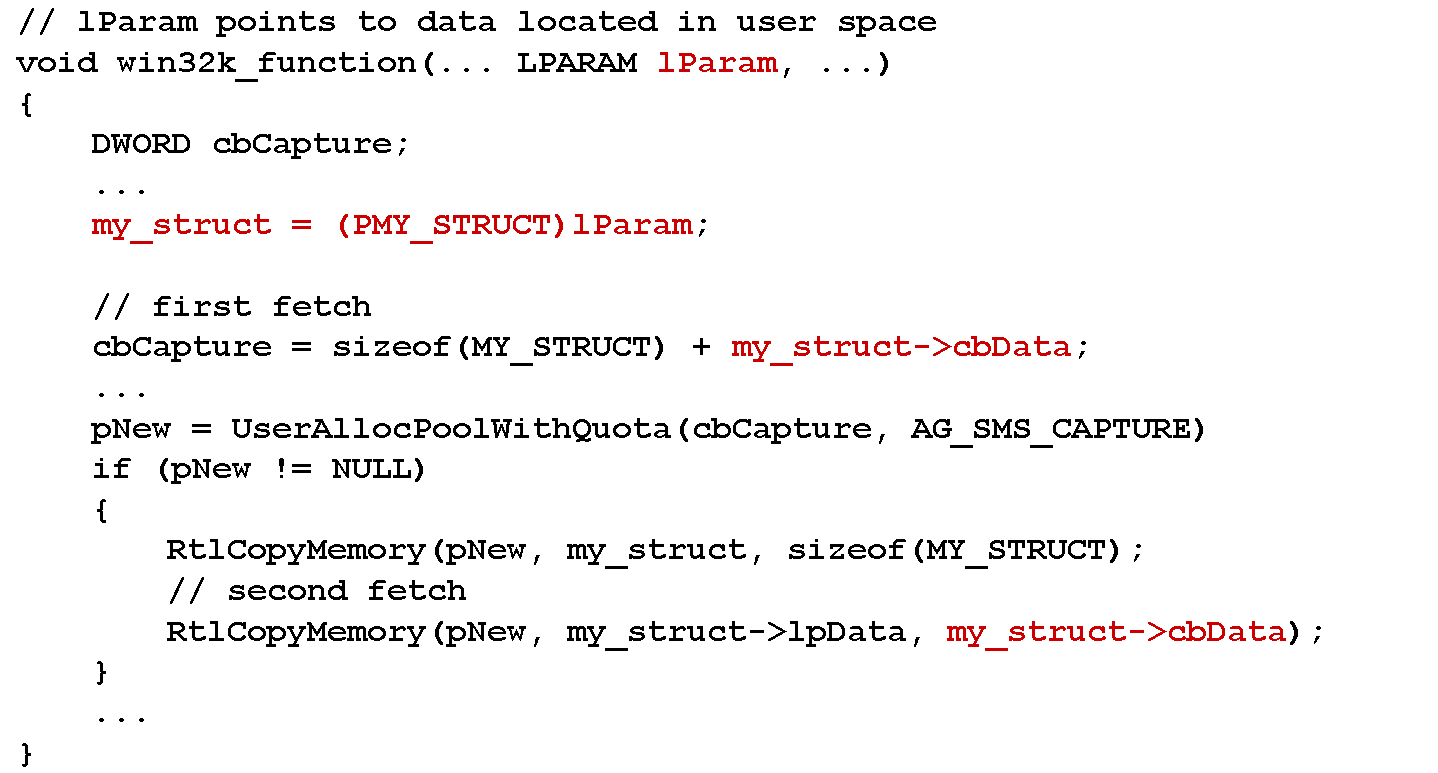
\includegraphics[width=0.47\textwidth]{figures/code08061}
	\centering
	\caption{Pseudocode of the vulnerability fixed in ms08-061. The vulnerable variable is in red. The kernel reads it twice, and it may get a different value for the buffer allocation and the subsequent buffer copying. It is common to see such a coding style. However, it is vulnerable because the two reads cross the privilege boundary.}
	\label{fig:code08061}
\end{figure}



~\autoref{fig:code08061} shows a piece of code from Windows Win32k module~\cite{jurczyk2013identifying}~\cite{ms08061}. This pseudo-code mimics a kernel-level TOCTOU vulnerability that has been identified and patched in ms08-061. It is part of the Win32k system call, and the code in red indicates the trace of the vulnerable code and data.  The user program passes \texttt{lParam} to \texttt{win32k\_function()} through upper layer API.  The first fetch occurs when summing up \texttt{cbCapture} with \texttt{my\_struct->cbData}, a data field offsetted from the address provided by \texttt{lParam}. The kernel allocates a buffer based on the data. However, shortly after, the kernel unnecessarily fetches this data again and uses it to copy data into the new buffer. As mentioned earlier, if the  \texttt{my\_struct->cbData} changes between the two fetches, especially when the last fetch gets a larger value, it will create a kernel heap buffer overflow. 

The attack time window is small, but enough. Even on a single processor system, the attack is feasible. For example, try to introduce a thread context switch between the two fetches. Because, for a local privilege escalation vulnerability like this, the attacker can invoke such a system call as many times as he needs. On a multi-processor system, the attacker usually creates another thread to race with the kernel, aiming at enlarging the data during the time window. As shown in~\autoref{fig:toctouasm}, the attacking thread 1 keeps flipping one higher bit of the variable. The attack succeeds by chance. If the latter value is smaller or equal to the former, the system will continue without error. If otherwise, the heap buffer overflow occurs.




\begin{figure}[ht]
  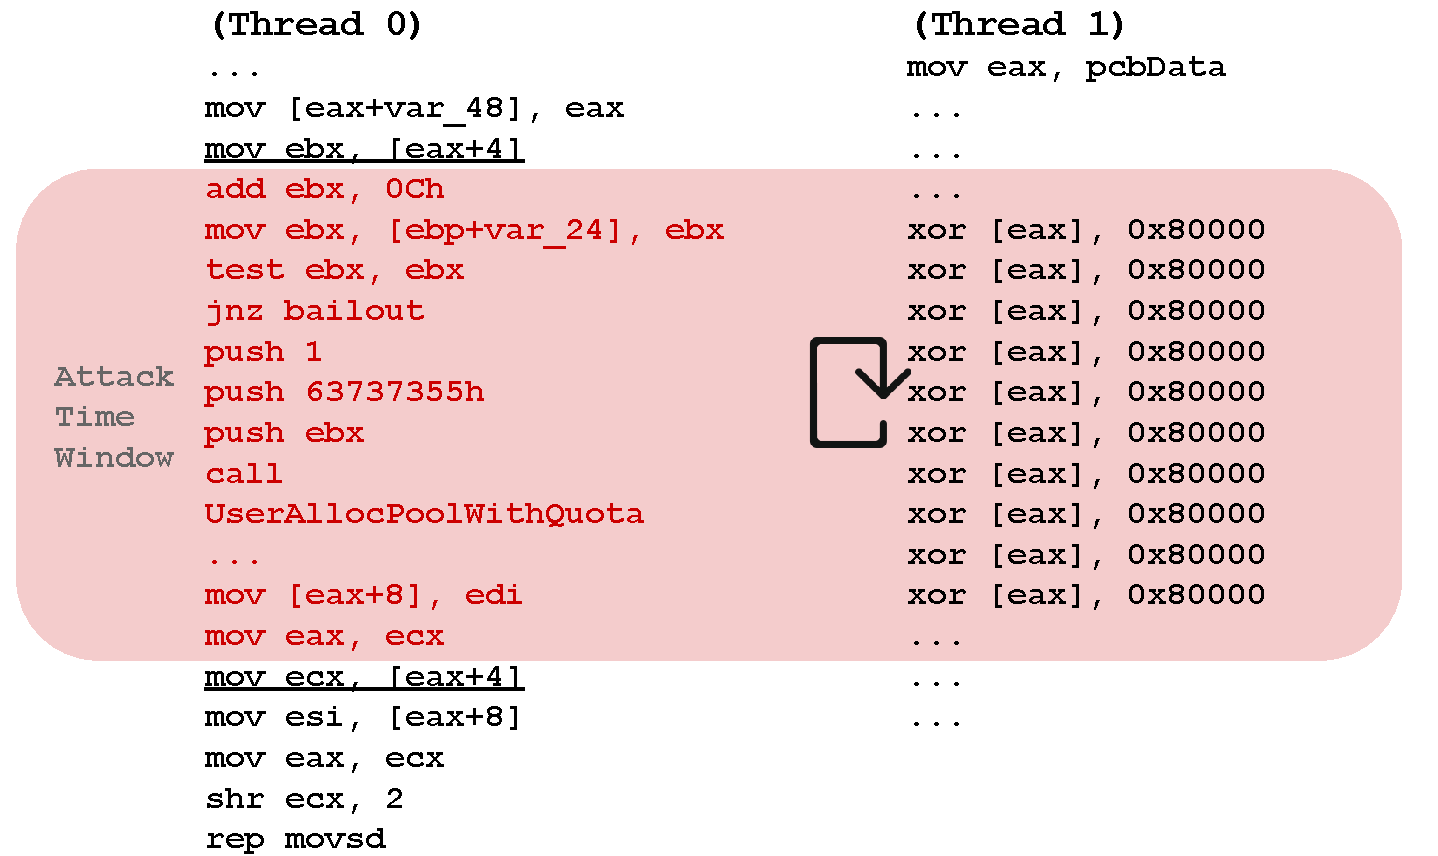
\includegraphics[width=0.47\textwidth]{figures/toctouasm3}
  \centering
  \caption{Thread 0 runs the vulnerable system call in the kernel-mode. The attacker can repeatedly call it to open the attack time window multiple times. Simultaneously, the other user-mode thread created by the attacker tries to flip the user-mode variable in-between the time window. So that the kernel code, two times, get the value differently.}
  \label{fig:toctouasm}
\end{figure}


%Once this step is accomplished, the problem becomes how to exploit it a classic heap buffer overflow. So you can see that kernel TOCTOU itself may not seems to be harmful, but it could lead to something serious. 

\subsection{Supervisor Mode Access Prevention (SMAP)}

%Kernel TOCTOU only needs accurate timing and memory writing, it's too plain to trigger any security mechanism so far. Existed monitoring methods are either too slow or too narrow, more details in~\autoref{sec:relatedwork}. We found a Intel CPU feature, Supervisor Mode Access Prevention (SMAP) is suitable for this task. 

%It's a security feature since Broadwell microarchitecture. It prevents operating system kernel directly accessing user-mode memory, which raises an exception. The intension is to stop transferring malicious payload from user space to kernel space.

%SMAP is enabled when the SMAP bit(21) in the CR4 is set. SMAP can be temporarily disabled for explicit memory accesses by setting the EFLAGS.AC (Alignment Check) flag. Because kennel does need to legally get data from user space, two more new instructions STAC (set AC flag) and CLAC (clear AC flag) are provided to accomplish that. The idea is that the kernel should be aware of when it's doing so. 

%For example, Linux kernel support for SMAP since version 3.7. All the accesses to user mode memory must go through two gateway functions \texttt{copy\_to\_user()} and \texttt{copy\_from\_user()}, where SMAP is temporarily disabled.

%However, Windows doesn't support SMAP yet. Different from Linux's approach, each of Windows syscalls tends to ``probe'' and ``capture'' user-mode data itself. Probing usually done by function ProbeForRead()~\cite{probeforread} and ProbeForWrite() to check the validity of the buffers, it also checks if a user mode buffer actually resides in the user space by simply compare its address to a pre-defined value. Since some modules such as win32k.sys are highly coupled with user-mode components, it will cost huge engineering effort to change the way it retrieve user-mode data.

%In Linux, even though \texttt{copy\_*\_user()} is mandated~\cite{corbet2012linuxsmap}, it still suffers from TOCTOU vulnerability such as mistake of using function \texttt{copy\_from\_user()} twice for the same variable~\cite{double-fetch-linux}. 



Monitoring the kernel's userspace behavior is essential to \name. Due to x86 protected mode characteristics, there is no mechanism available for a broad range of monitoring memory modifications. Techniques such as leveraging hardware watchpoints or transactional memory are fittable for fuzzing such vulnerabilities in a small memory range. However, none of them is realistic for run-time system protection. We discuss more details in~\autoref{sec:experiment} and~\autoref{sec:relatedwork}.

Fortunately, we notice an Intel CPU feature so-called \texttt{Supervisor Mode Access Prevention (SMAP)}~\cite{corbet2012supervisorsmap}~\cite{mulnix2016intel} accurately serves the purpose.
\texttt{SMAP} is a feature since the Intel Broadwell microarchitecture prevents the kernel from freely accessing userspace so that such access will raise an exception. It complements \texttt{Supervisor Mode Execution Prevention (SMEP)}~\cite{fischer2011supervisor} that introduced earlier. \texttt{SMEP} can be used to prevent the kernel from unintentionally executing user-mode code. \texttt{SMAP} extends this protection to reads and writes. It makes it harder for a malicious program to deceive the kernel into using code or data from the userspace.

\texttt{SMAP} is enabled when \texttt{CR4.SMAP} sets to 1. SMAP can be temporarily disabled for direct memory accesses by setting the \texttt{EFLAGS.AC} flag, and the \texttt{stac} and \texttt{clac} instructions set or clear the flag. Doing so indicates that the kernel is fully aware the userspace-access behavior. For example, Linux kernel supports \texttt{SMAP} since version 3.7. The kernel-to-userspace accesses must go through two gateway functions \texttt{copy\_to\_user()} and \texttt{copy\_from\_user()}, in which \texttt{SMAP} is temporarily disabled.

However, Windows does not support \texttt{SMAP} still. It takes a different approach: ``probe'' and ``capture'' user-mode data from each system call. \texttt{ProbeForRead()}~\cite{probeforread} and \texttt{ProbeForWrite()} validates user-mode buffer. It also checks whether the buffer belongs to userspace by comparing the buffer address to a pre-defined value. This mechanism is effective if done correctly and thoroughly. However, kernel components such as Win32k still failed to practice the ``probe'' and ``capture'' in a large portion of their code. Because Win32k still couples with user-mode components, it will cost huge engineering effort to change how it directly access user-mode data.
